\section{Risultati}\label{sec:risultati}

\subsection{Esecuzione ideale}

Nel caso ideale, l'algoritmo è stato eseguito
simulando il sistema quantistico tramite \texttt{statevector\_simulator}, 
senza la presenza di rumore. L'immagine originale,
elaborata tramite il simulatore, produce il risultato mostrato in
Fig.~\ref{fig:statevector-detection}. Questo risultato evidenzia chiaramente i bordi
dell'immagine con un'elevata precisione, grazie all'assenza di fattori
disturbanti come il rumore o le imperfezioni hardware. Questo scenario
rappresenta il limite teorico dell'algoritmo, fornendo una base di confronto per
valutare le prestazioni in condizioni più realistiche.

\begin{figure}
	\centering
	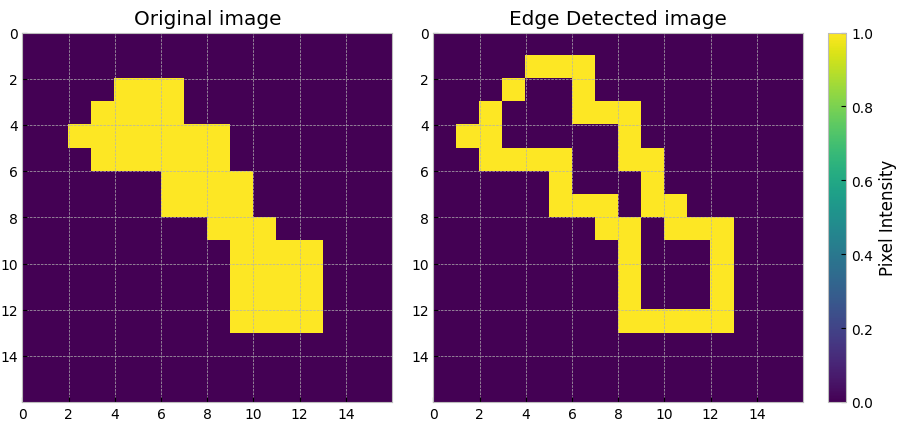
\includegraphics[width=0.45\textwidth]{statevector-detection.png}
	\caption{Risultato dell'elaborazione tramite \texttt{state\_vector}.}
	\label{fig:statevector-detection}
\end{figure}

\subsection{Esecuzione con rumore simulato}

Per valutare il comportamento dell'algoritmo in condizioni più vicine alla
realtà, è stato introdotto un modello di rumore (\texttt{NoiseModel}) basato
sull'hardware reale \texttt{ibm\_kyiv}. In questo caso, l'esecuzione quantistica
tiene conto di fattori come decoerenza e errori di lettura, che sono comuni nei
dispositivi quantistici attuali.

La Fig.~\ref{fig:16x16-shots} mostra il risultato dell'elaborazione con
l'inclusione del rumore, variando il numero di \textit{shots} (ossia il numero
di ripetizioni dell'esecuzione del circuito quantistico). Si osserva che un
numero maggiore di shots migliora il rilevamento dei bordi; inoltre, il
risultato finale non mostra particolari differenze rispetto al caso ideale. È
interessante notare che è possibile ottenere una buona approssimazione dei
contorni dell'immagine già a partire da 4096 shots.

\begin{figure}[ht]
	\centering
	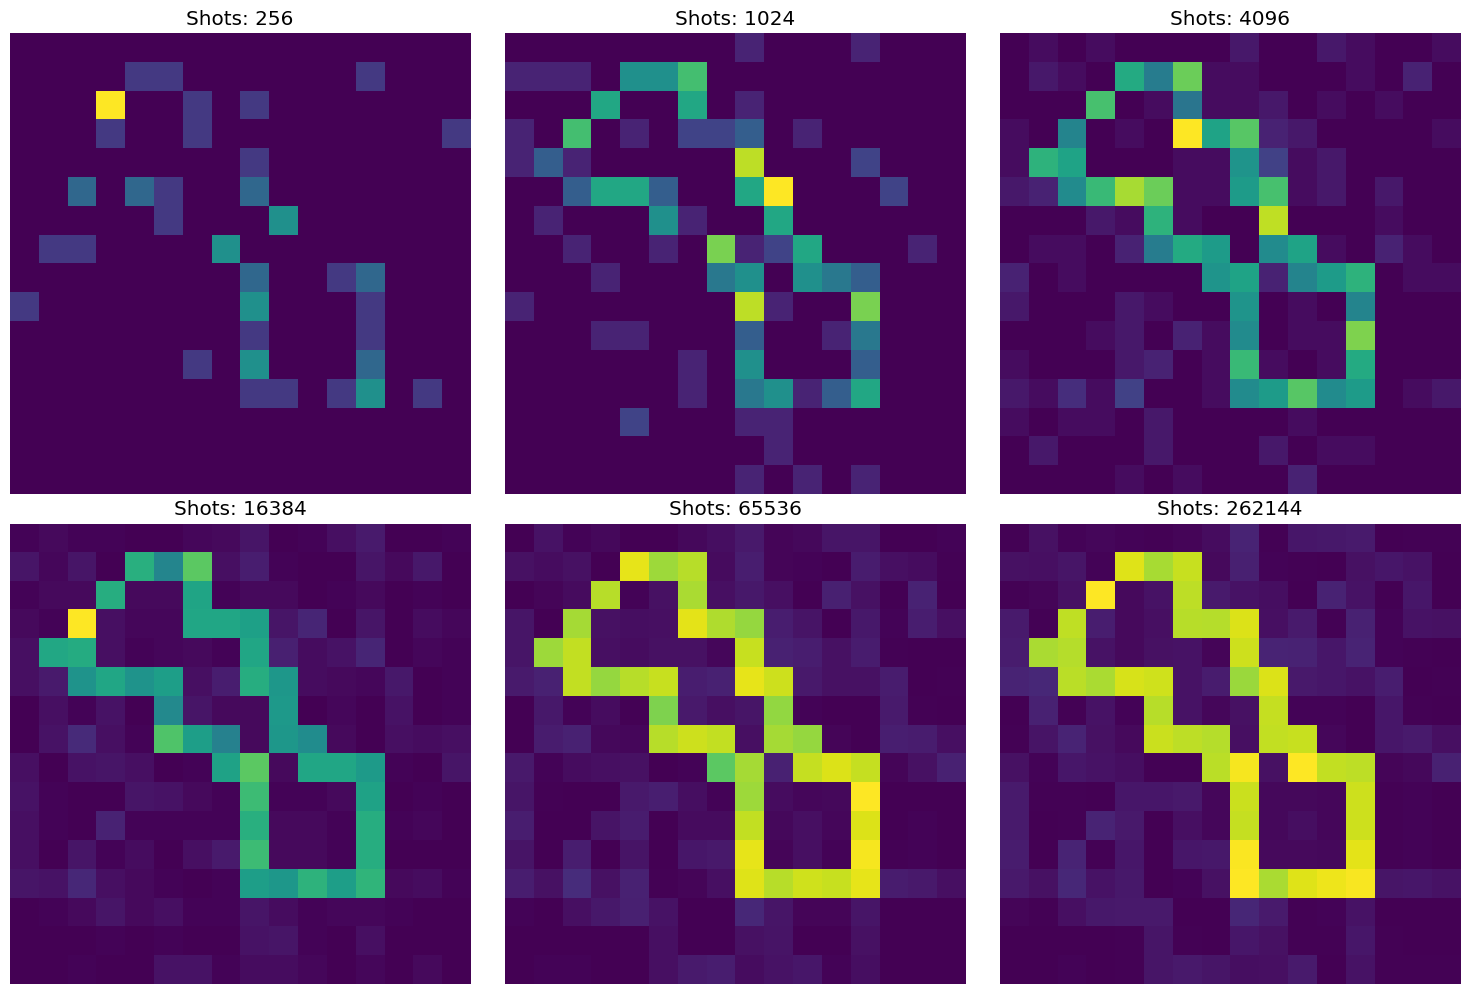
\includegraphics[width=0.9\columnwidth]{16x16-shots.png}
	\caption{Risultato dell'elaborazione utilizzando \texttt{NoiseModel} con numero di shots differenti.}\label{fig:16x16-shots}
\end{figure}

\subsection{Esecuzione del circuito ``transpiled''}
È stato possibile eseguire il transpiling soltanto di circuiti relativi a
immagini $2 \times 2$. Utilizzando il
parametro \texttt{optimization\_level=3}, la versione ``transpiled'' del circuito
rappresentato in Fig.~\ref{fig:circuito-2x2} risulta avere profondità 64. 
In Fig. \ref{fig:2x2-simulation} e \ref{fig:2x2-shots} viene mostrata 
l'immagine originale, seguita dalle rispettive simulazioni, con e senza rumore.
Viste le dimensioni ridotte dell'immagine, l'esecuzione
con diverse soglie di shots non sembra essere particolarmente significativa.
Nonostante questo, si può dire che il comportamento del circuito è corretto, 
poiché i risultati coincidono con le misurazioni ottenute tramite \texttt{state\_vector}.

\begin{figure}[ht]
	\centering
	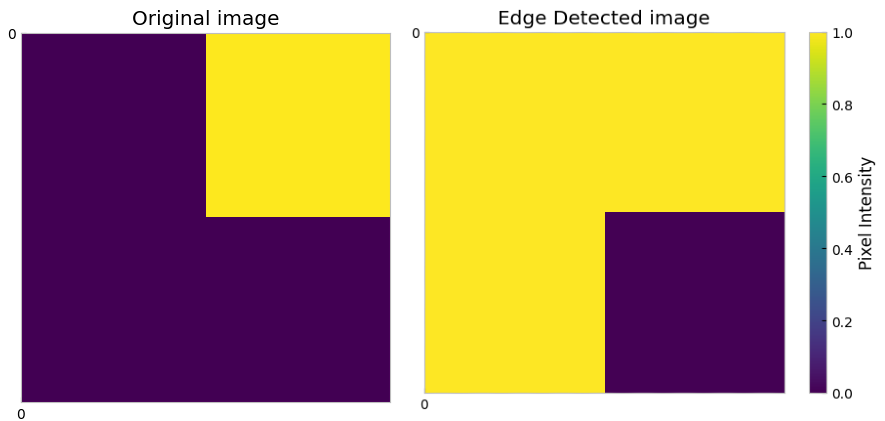
\includegraphics[width=0.9\columnwidth]{2x2-simulation.png}
	\caption{Esempio di immagine $2\times2$.}\label{fig:2x2-simulation}
\end{figure}

\begin{figure}[ht]
	\centering
	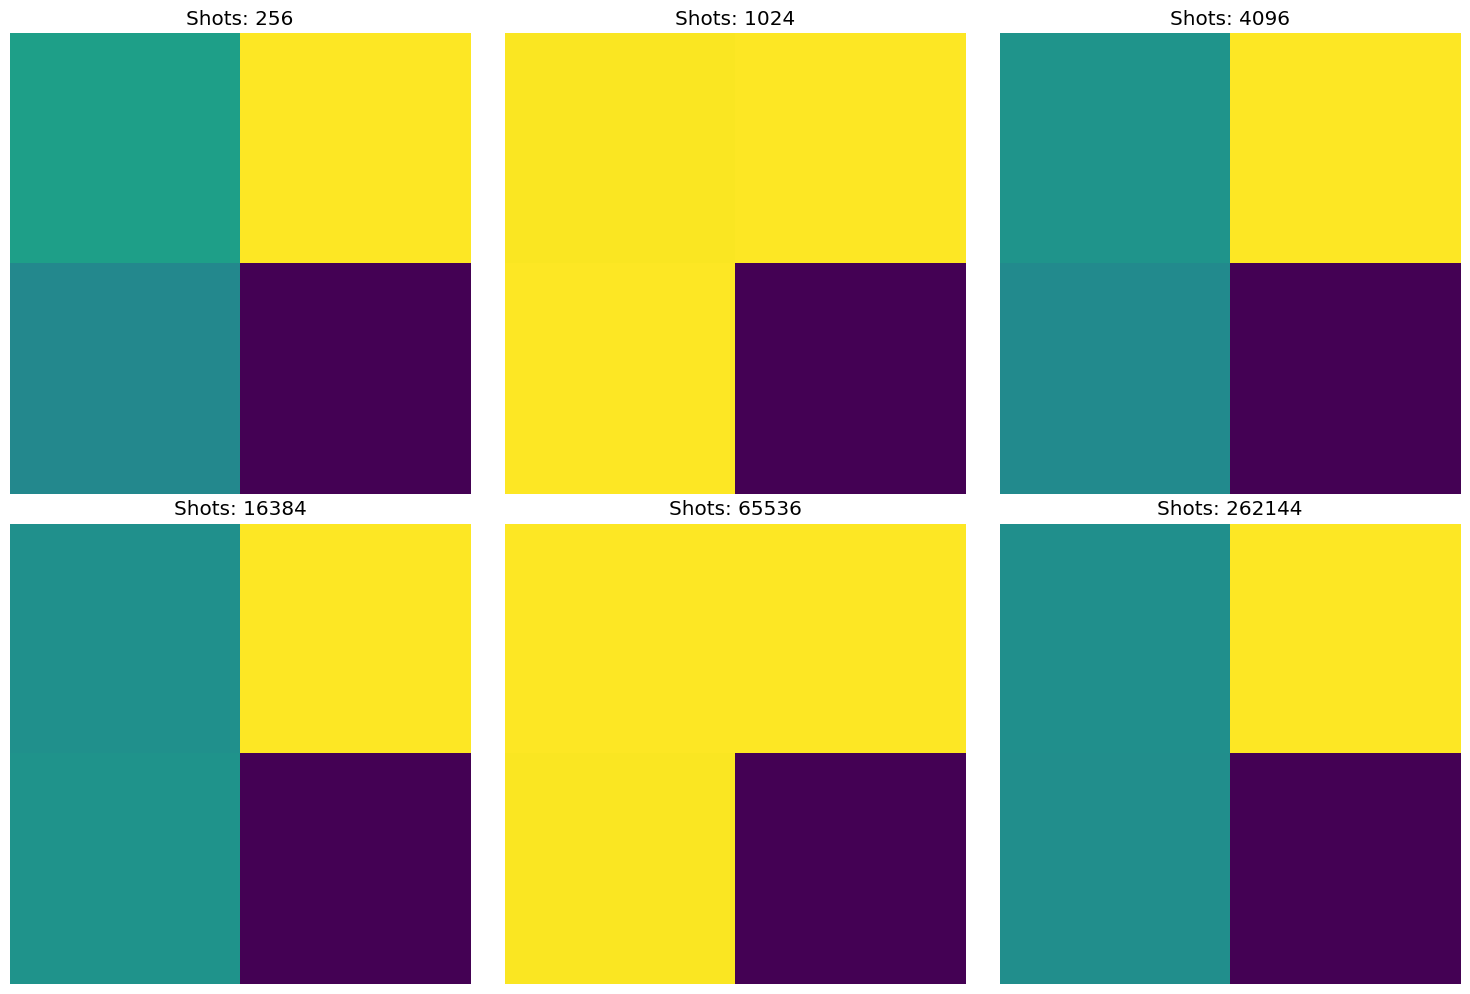
\includegraphics[width=0.9\columnwidth]{2x2-shots.png}
	\caption{Risultato dell'elaborazione sul circuito transpiled, 
	utilizzando \texttt{NoiseModel} con numero di shots differenti 
	su immagine $2\times2$.}\label{fig:2x2-shots}
\end{figure}

